\section{Conclusion}

\begin{frame}{\acs{AI} now and tomorow in Science}
  \begin{itemize}
  \item Combine Symbolic and Neural Networks:
    \begin{itemize}
    \item \textbf{Combine NN and symbolic representations} \note{integrating a priori knowledge of the scientific domain}
    \item \textbf{Incorporating Prior Knowledge} \note{Embedding symbolic, pre-existing knowledge (like ontologies) into neural networks to guide learning}
      \note{\textbf{Enhancing Interpretability} Symbolic knowledge helps in making the models more interpretable and trustworthy}
    \item \textbf{Integration} of neuro-symbolic engine and multi-level representations
    \item \textbf{AlphaGeometry}
    \end{itemize}

  \item Learn from heterogeneous data:
    \begin{itemize}
      \note{originating from various
        sensors in embedded systems (robotics, aerospace), from different detector subsystems /instruments or from different signal sources in a scientific
        experiment in general}
    \item Scientific data often \textbf{heterogeneous and multimodal} in nature
    \item \textbf{Learn shared latent representations}
    \item Enhance model's capacity to \textbf{represent} the data
    \item \textbf{Polymathic AI}
    \end{itemize}
  \end{itemize}
\end{frame}

% Challenges
\begin{frame}
  \note{
    \begin{itemize}
    \item Provide some insights on data hell
    %\item How would you rate GW data?
    \item Challenges in particular theoretical development
    \end{itemize}
  }
  \frametitle{Challenges}

  \begin{textblock}{90}(5, 10)
    \begin{itemize}
    \item Obtaining good data is hard:
      \begin{itemize}
      \item Challenges of ``big data'': volume, velocity, variety, veracity (4V)
      \item Systematic biases
      \item Legal issues: GDPR, sensitive research, confidentiality
      \item Data acquisition, cleaning and normalization can take up to 80\% of
        the time
      \end{itemize}
    \item \acl{xAI}:
      \begin{itemize}
      \item Opening the black-box
      \item Interpretability: begin able to build indicators on the decision of the model
        (which variables are the most important, understand parts of the model)
      \item Explicability: being able to explain the decision of the model
      \end{itemize}
    \item Ethical \ac{AI}:
      \begin{itemize}
      \item How to build systems which respect fundamental values like individual rights, privacy, non-discrimination and non-manipulation?
      \end{itemize}
    \item More technical challenges:
      \begin{itemize}
      \item Unsupervised learning
      \item New protocols: online learning, active learning
      \item Reproductibility
      \item Not just predict but \emph{understand} the data
      \end{itemize}
    \end{itemize}
  \end{textblock}
\end{frame}


\begin{frame}
  \frametitle{See you soon in Toulouse!}
  \begin{center}\LARGE AISSAI Workshop: Heterogeneous Data and Large Representation Models in Science\end{center}
  \begin{center}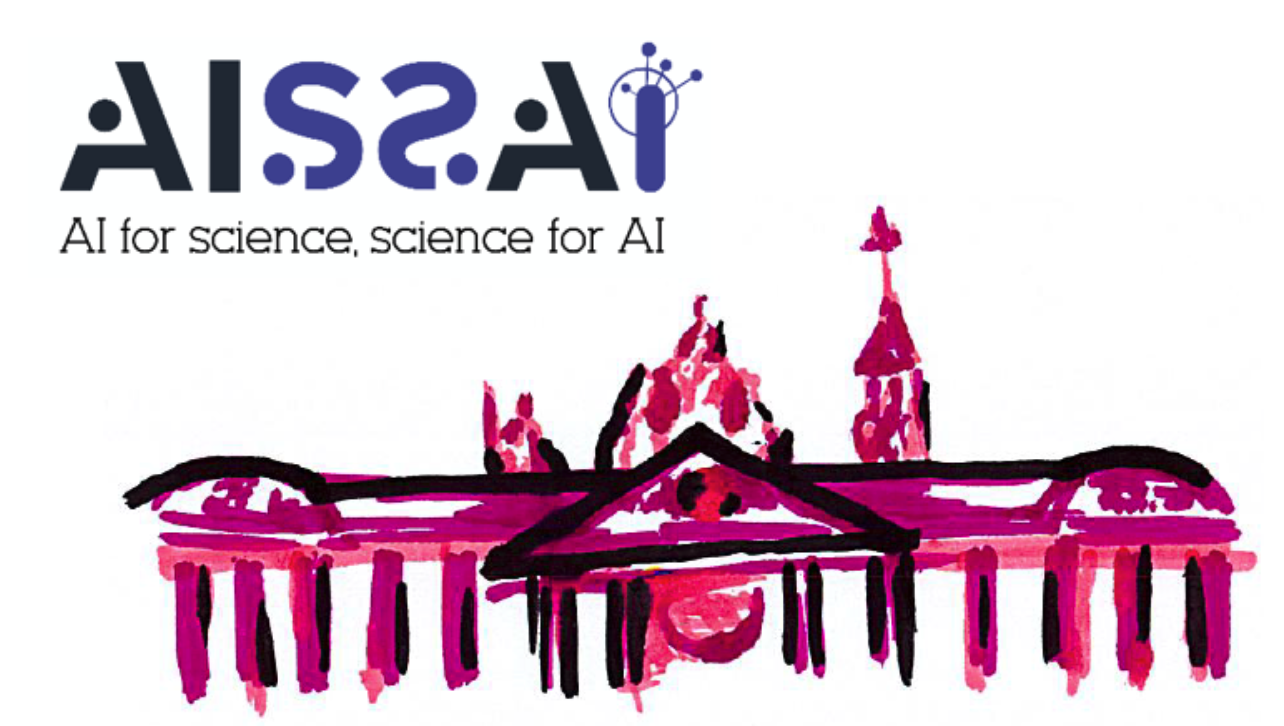
\includegraphics[width=200px]{img/invitation.png}\end{center}

  \begin{center}\large from September 30 to October 3rd, 2024\end{center}
  \begin{center}\large \url{https://indico.in2p3.fr/event/33412/}\end{center}
  % \begin{center}\Large See you soon in Toulouse!\end{center}
\end{frame}
